\chapter{Model Design}

\section{Introduction}

\section{Objectives}
The main objective

\section{Properties}
\label{section:ModelDesign:Properties}
We expect the model $\mathcal{M}$ to verify the following properties:

\subsection{Totality}
\subsubsection{Definition}
A function is total if it is defined in the whole domain.
\newline Also, we will say a model $\mathcal{M}$ is total if it works on all Mean Payoff Games..
\subsubsection{Importance}
This property implies two main characteristics:
\begin{enumerate}
	\item The model works for any Mean Payoff Game whatever the size of $\lvert \VertexSet \rvert.$ This is difficult to not violate, as most machine learning models require static shapes.
	\item The model works for any Mean Payoff Game whatever the representation is; This is implicitely verified by an encoding of the Mean Payoff Games.
\end{enumerate}

\subsection{Node Agnostic}
This property tells that a model should not use any extra information about the nodes.
\subsubsection{Formalisation}
Let $G_1(V_1,E_1,W_1,s_1),G_2(V_2,E_2,W_2,s_2)$ two isomorphic Mean Payoff Games in the sense that there exists a bijection $\Phi:V_1\rightarrow V_2$ such that:
\begin{align*}
	E_2&=\{(\Phi(u),\Phi(v)),\quad (u,v)\in E_1\}\\
	\forall (u,v)\in E_1,\quad W_2(u,v)&=W_1(\Phi(u),\Phi(v)) \\
	s_2&= \Phi(s_1)
\end{align*}
Then:
$$
\Phi\left(\mathcal{M}(G_1)\right) = \mathcal{M}(G_2)
$$
\subsubsection{Explanation}
The property tells that if two graphs mean payoffs only differ by their node representation, then the results should also only differ by the representation of the nodes.

\subsubsection{Importance}
This property implies that we can simply encode a mean payoff as $G(V,E,W,s)$ as $G'(V',E',W',s')$ with  $V'=\{0,\dot,\lvert V \rvert-1\},$ and $E',W',s'$ defined accordingly.
\newline In fact, the encoding is done implicitely by our model\footnote{While the encoding is done implicitely, the model itself can violate this property. An example of this is a Multi Layer Perceptron. Which lead to different results for different encodings.}.

\begin{figure}[H]
	\begin{subfigure}[b]{0.3\textwidth}
		\begin{tikzpicture}[->,>=stealth',shorten >=1pt,auto,node distance=2cm,
			thick,main node/.style={circle,draw,font=\Large\bfseries}]
			\node[main node, fill=gray!50] (1) {$2$}; 
			\node[main node] (2) [right of =1] {$3$}; 
			\node[main node] (3) [above right of =1] {$0$}; 
			\node[main node] (4) [right of =2] {$1$}; 
			\path (1) edge [bend left] node {1} (3)
			edge [bend right] node [below] {-1} (2)
			(2) edge [bend right] node [above] {1} (1)
			edge [loop below] node {-1} (2)
			(3) edge [bend left] node {-5} (2)
			edge [bend left] node {-2} (4)
			(4) edge node {3} (2);
		\end{tikzpicture} 
	\end{subfigure}
	\hfill
	\begin{subfigure}[b]{0.3\textwidth}
		\begin{tikzpicture}[->,>=stealth',shorten >=1pt,auto,node distance=2cm,
			thick,main node/.style={circle,draw,font=\Large\bfseries}]
			\node[main node, fill=gray!50] (1) {$0$}; 
			\node[main node] (2) [right of =1] {$1$}; 
			\node[main node] (3) [above right of =1] {$2$}; 
			\node[main node] (4) [right of =2] {$3$}; 
			\path (1) edge [bend left] node {1} (3)
			edge [bend right] node [below] {-1} (2)
			(2) edge [bend right] node [above] {1} (1)
			edge [loop below] node {-1} (2)
			(3) edge [bend left] node {-5} (2)
			edge [bend left] node {-2} (4)
			(4) edge node {3} (2);
		\end{tikzpicture}
	\end{subfigure} 
	\hfill
	\begin{subfigure}[b]{0.3\textwidth}
		\begin{tikzpicture}[->,>=stealth',shorten >=1pt,auto,node distance=2cm,
			thick,main node/.style={circle,draw,font=\Large\bfseries}]
			\node[main node, fill=gray!50] (1) {\scriptsize Cat}; 
			\node[main node] (2) [right of =1] {\scriptsize Dog}; 
			\node[main node] (3) [above right of =1] {\small Yak}; 
			\node[main node] (4) [right of =2] {\scriptsize Fox}; 
			\path (1) edge [bend left] node {1} (3)
			edge [bend right] node [below] {-1} (2)
			(2) edge [bend right] node [above] {1} (1)
			edge [loop below] node {-1} (2)
			(3) edge [bend left] node {-5} (2)
			edge [bend left] node {-2} (4)
			(4) edge node {3} (2);
		\end{tikzpicture} 
	\end{subfigure}
	\caption{Three isomorphic Mean Payoff Games}
	\label{fig:NodeAgnostic}
\end{figure}
\FloatBarrier
In the figure \ref{fig:NodeAgnostic}, we have $3$ equivalent Mean Payoff Games.
To illustrate a node agnostic model:
\begin{itemize}
	\item Let $\mathcal{M}$ be a model that predicts for a given Mean Payoff Game, the action to be played at the starting node, and the winner.
	\item Suppose also that $\mathcal{M}(G_1)=(3,\text{Max})$
\end{itemize}
If $\mathcal{M}$ is node agnostic, then:
\begin{align*}
	\mathcal{M}(G_2)&=(1,\text{Max})\\
	\mathcal{M}(G_3)&=(\text{Dog},\text{Max})
\end{align*}
\subsection{Invariance under Positive Scaling}
\label{section:ModelDesign:Properties:Invariance}
This property comes directly from the fact that both the winner and the set of optimal strategies\footnote{Whatever the definition of optimality (Weak, Strong, Payoff).} are invariant under a positive scaling of the weights.
\newline
Now, it is very easy to make augment a model $\mathcal{M}$ into such invariant model $\mathcal{M}'.$ We only do the following:
$$
\mathcal{M}'(E,W,s)=\mathcal{M}'(E,\text{Normalize}(W),s)
$$
Where $\text{Normalize}$ is any endomorphism of weight functions that verify the following constraint:
$$
\forall_{\text{MPG}}G(E,W),\forall ,\quad \text{Normalize}(W)=\frac{W}{H(W)}
$$
With $H:\mathscr{F}(E,\mathbb{R})\rightarrow \mathscr{F}(E,\mathbb{R})$ a function satisfying\footnote{Special care must be when $H$ is $\ge$ instead of $>$}:
\begin{align*}
	\forall s\in\mathbb{R}_+^*,\quad H(sW)&=sH(W) \\
	H(W)&> 0
\end{align*}

\subsubsection{Standard Scaling}
This scaling treats the values of $W$ as samples of random variables, and divides $W$ by an estimate of their variance. 
\begin{align*}
	\text{Normalize}(W)&=\frac{W}{\sqrt{\mathbb{V}[W]}}\\
	\mathbb{V}[W]&=\frac{1}{\lvert E \rvert} \sum_{(u,v)\in E}(W(u,v)-\mathbb{E}[W])^2 \\
	\mathbb{E}[W]&=\frac{1}{\lvert E \rvert}\sum_{(u,v)\in E}W(u,v) 
\end{align*}



\subsubsection{Maximum Scaling}
This scaling reduces the interval of the weights to $[-1,1]$ by dividing by the largest weight in terms of absolute value:
$$
\text{Normalize}(W)=\frac{W}{\lVert W \rVert_{\infty}}
$$
\paragraph{Implementation Notes:}
The weights function is implemented as a matrix $W,$ which is equal to $0$ for $(u,v)\notin E.$ 
\newline It is important to igonre these zeros\footnote{And only these zeros. If $W(u,v)=0$ for $(u,v)\in E$, this term should be accounted.} in both normalisations, otherwise it may lead to biased scaling.

\begin{figure}[H]
	\begin{subfigure}[b]{0.45\textwidth}
		\raggedleft
		\begin{tikzpicture}[->,>=stealth',shorten >=1pt,auto,node distance=2cm,
			thick,main node/.style={circle,draw,font=\Large\bfseries}]
			\node[main node, fill=gray!50] (1) {$2$}; 
			\node[main node] (2) [right of =1] {$3$}; 
			\node[main node] (3) [above right of =1] {$0$}; 
			\node[main node] (4) [right of =2] {$1$}; 
			\path (1) edge [bend left] node {1} (3)
			edge [bend right] node [below] {-1} (2)
			(2) edge [bend right] node [above] {1} (1)
			edge [loop below] node {-1} (2)
			(3) edge [bend left] node {-5} (2)
			edge [bend left] node {-2} (4)
			(4) edge node {3} (2);
		\end{tikzpicture} 
	\end{subfigure}
	\hfill
	\begin{subfigure}[b]{0.45\textwidth}
		\raggedright
		\begin{tikzpicture}[->,>=stealth',shorten >=1pt,auto,node distance=2cm,
			thick,main node/.style={circle,draw,font=\Large\bfseries}]
			\node[main node, fill=gray!50] (1) {$2$}; 
			\node[main node] (2) [right of =1] {$3$}; 
			\node[main node] (3) [above right of =1] {$0$}; 
			\node[main node] (4) [right of =2] {$1$}; 
			\path (1) edge [bend left] node {0.2} (3)
			edge [bend right] node [below] {-0.2} (2)
			(2) edge [bend right] node [above] {0.2} (1)
			edge [loop below] node {-0.2} (2)
			(3) edge [bend left] node {-1} (2)
			edge [bend left] node {-0.4} (4)
			(4) edge node {0.6} (2);
		\end{tikzpicture} 
	\end{subfigure}
	\caption{Mean Payoff Game, with a rescaled version using Maximum normalization}
\end{figure}

\subsection{Permutation Equivariance}
\subsubsection{Definition}
This property states that the model should ouptut the same results for permuted nodes, up to permutation of the results.
\subsubsection{Importance}
While it is a special case of the Node Agnostic property, but it is still important as the encoding of the graphs is done implicitely, and thus Permutation Equivariance is enough to get a Node Agnostic model.
\subsection{Stability under Padding}
\subsubsection{Definition}
Let $G_1(V_1,E_1,W_1,s_1),G_2(V_2,E_2,W_2,s_2)$ be two disjoint Mean Payoff Games, in the sense that $V_1\cap V_2=\varnothing.$
\newline The padding of $G_1$ by $G_2,$ denoted $G_1\rhd G_2$ defined as:
$$
G_1\rhd G_2=(V_1\cup V_2,E_1\cup E_2,W_1\cup W_2,s_1)
$$
A model is said to be stable under padding if:
$$
\mathcal{M}(G_1\rhd G_2)=\mathcal{M}(G_1)
$$
\subsubsection{Importance}
Deep Learning algorithms generally accept batches of data having a homogeneous shape.
\newline In the other hand, graph input generally has different shapes, and thus are problematic to most learning algorithms.
\newline While we succeeded in experimenting a learning algorithm with a ragged batch\footnote{A batch of inhomogeneous input}, it suffered the following limits:
\begin{itemize}
	\item It greatly limits the choice of potential models. 
	\item The training is not supported by GPU, as some core operations were only implemented in the CPU for ragged batches.
\end{itemize}
For this reasons, we opted to pad the graphs to get homogeneous batches, and this is why the stability under padding is important.
\subsubsection{Removing Unreachable Nodes}
Another major point for this property, is it gives the possibility to remove unreachable nodes\footnote{If we ignore the orientation. A stronger property allowing unreachable nodes on the di-graph can also be defined, but this is beyond the scope.} without affecting the model's results.

\begin{figure}[H]
	\begin{subfigure}[b]{0.45\textwidth}
		\raggedleft
		\begin{tikzpicture}[->,>=stealth',shorten >=1pt,auto,node distance=2cm,
			thick,main node/.style={circle,draw,font=\Large\bfseries}]
			\node[main node, fill=gray!50] (1) {$2$}; 
			\node[main node] (2) [right of =1] {$3$}; 
			\node[main node] (3) [above right of =1] {$0$}; 
			\node[main node] (4) [right of =2] {$1$}; 
			\path (1) edge [bend left] node {0.2} (3)
			edge [bend right] node [below] {-0.2} (2)
			(2) edge [bend right] node [above] {0.2} (1)
			edge [loop below] node {-0.2} (2)
			(3) edge [bend left] node {-1} (2)
			edge [bend left] node {-0.4} (4)
			(4) edge node {0.6} (2);
		\end{tikzpicture} 
	\end{subfigure}
	\hfill
	\begin{subfigure}[b]{0.45\textwidth}
		\raggedright
		\begin{tikzpicture}[->,>=stealth',shorten >=1pt,auto,node distance=2cm,
			thick,main node/.style={circle,draw,font=\Large\bfseries}]
			\node[main node, fill=gray!50] (1) {$2$}; 
			\node[main node] (2) [right of =1] {$3$}; 
			\node[main node] (3) [above right of =1] {$0$}; 
			\node[main node] (4) [right of =2] {$1$}; 
			
			\node[main node] (7) [below of =2] {$7$}; 
			\node[main node] (5) [below left of =7] {$4$}; 
			\node[main node] (6) [below right of =7] {$5$}; 
			\path (1) edge [bend left] node {1} (3)
			edge [bend right] node [below] {-1} (2)
			(2) edge [bend right] node [above] {1} (1)
			edge [loop below] node {-1} (2)
			(3) edge [bend left] node {-5} (2)
			edge [bend left] node {-2} (4)
			(4) edge node {3} (2)
			(5) edge node {-3} (7)
			(6) edge node {5} (5)
			(7) edge node {0} (6);
		\end{tikzpicture} 
	\end{subfigure}
	\caption{Original Mean Payoff Game with a padded version}
	\label{fig:StableUnderPadding}
\end{figure}
\FloatBarrier
Following the example under figure \ref{fig:StableUnderPadding}, if the model $\mathcal{M}$ is stable under padding, then the triangular subgraph should not be accounted in the output.
\section{Considered Models}
While there are many possible predictive models. We considered mainly two families of predictive models.
\subsection{Value based Model}
Such model predicts the evaluation of a certain position.
\newline The evaluation is a function $\mathcal{M}:\VertexSet \times \PlayerSet \rightarrow [-1,1]$ with the following interpretation:
\begin{itemize}
	\item $\mathcal{M}(s,p)=1$ when the model predicts that player $p$ will win the game given the position.
	\item $\mathcal{M}(s,p)=-1$ whens the model predicts that player $p$ will lose the game given the position.
	\item $\mathcal{M}(s,p)=0$ when the model predicts that the position will result in a draw.
\end{itemize}
Now, while such a model can be used to predict the winner. We claim that it is not efficient\footnote{Efficient in the sense that we cannot extract the best strategy from the evaluation in linear time.} to extract the strategy from such model, as the information of winning alone does not directly induce a strategy.
\newline The following figure illustrates an example.
\begin{figure}
	\centering
	\begin{tikzpicture}[->,>=stealth',shorten >=1pt,auto,node distance=4cm,
		thick,main node/.style={circle,draw,font=\Large\bfseries}]
		\node[main node] (5) {$5$};
		\node[main node, fill=gray!50] (1) [below left of =5] {$0$}; 
		\node[main node] (2) [below right of =5] {$1$}; 
		\node[main node] (3) [above right of =5] {$2$}; 
		\node[main node] (4) [above left of =5] {$3$}; 
		\path (1) edge [bend left=12] node {1} (5)
				  edge node {-1} (2)
		(2) edge node {-1} (3)
		edge [bend left=12] node {1} (5)
		(3) 
		edge [bend left=12] node {1} (5)
		edge node {-1} (4)
		(4)
		edge node {-1} (1)
		edge [bend left=12] node {1} (5)
		(5) edge [bend left=12] node {1} (1)
			edge [bend left=12] node {1} (2)
			edge [bend left=12] node {1} (3)
			edge [bend left=12] node {1} (4);
			
	\end{tikzpicture} 
	\caption{An MPG where the first player always wins.}
\end{figure}
\FloatBarrier
\subsection{Strategy based Model}
Such model predicts the strategy for each player.
\newline This is a function $\mathcal{M}:\VertexSet \times \PlayerSet \rightarrow \mathscr{P}(\VertexSet)$ such that:
\begin{align*}
	\forall (u,p)\in \VertexSet \times \PlayerSet, \quad \mathcal{M}(u,p) &\in \Adj u \\
	\forall (u,p) \in \VertexSet \times \PlayerSet,\forall v \in \Adj u, \quad  \mathcal{P}\left(\mathcal{M}(u,p) =v \right)  &\in [0,1] \\ 
\forall (u,p) \in \VertexSet \times \PlayerSet, \quad  \sum_{v\in \Adj u}\mathcal{P}\left(\mathcal{M}(u,p) =v \right) &=1 \\ 
\end{align*}
\section{Building the Model}
Our model follows from well esta../Figures/PreprocessingBlock.pngblished graph neural network architectures, with minor modifications to suit our needs.
\newline It is composed of blocks, each containing a \textbf{Weighted Graph Convolutional Network}.
\subsection{Weighted Graph Convolutional Network}
The weighted graph convolutional network \textbf{WGCN}, as its name suggests, is a convolutional operator acting on graphs, with many desirable properties such as ``Permutation Equivariance" and ``Stability under Padding".
\newline It is based on the graph convolutional network as described on the following figure
\begin{figure}[H]
	\noindent
	
	\makebox[\textwidth]{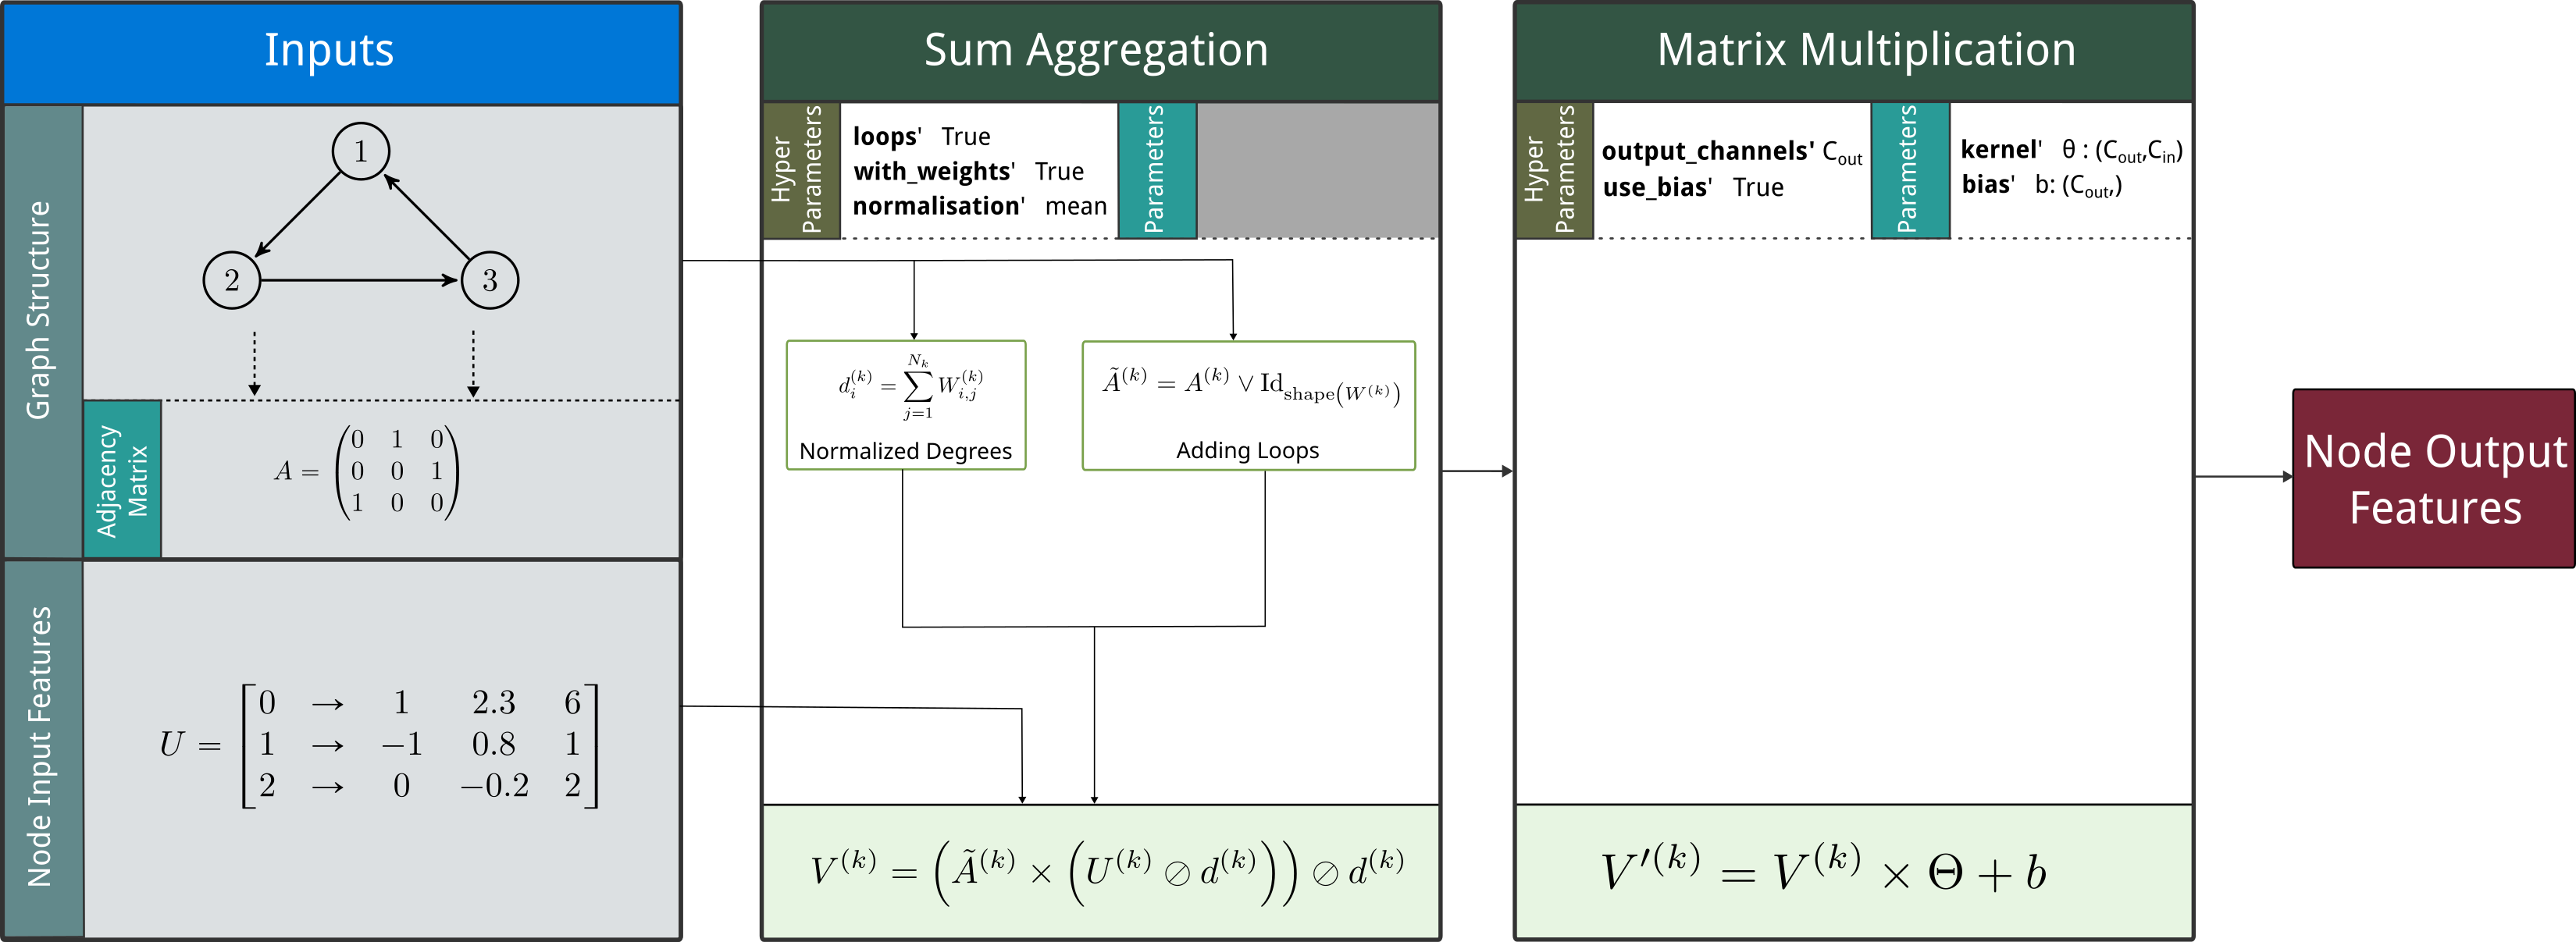
\includegraphics[width=1.2\textwidth]{Figures/GCN.png}}
	\caption{Graph Convolutional Network}
	\label{fig:GCN}
\end{figure}
\FloatBarrier
The problem with \textbf{GCN} is that they ignore the weights information. For Mean Payoff Games, such information is crucial to determine the winner and the strategies.
\newline For that, we introduced \textbf{WGCN} to capitalize on the weights information. The figure below shows how it is implemented.

\begin{figure}[H]
	  \noindent
	
	\makebox[\textwidth]{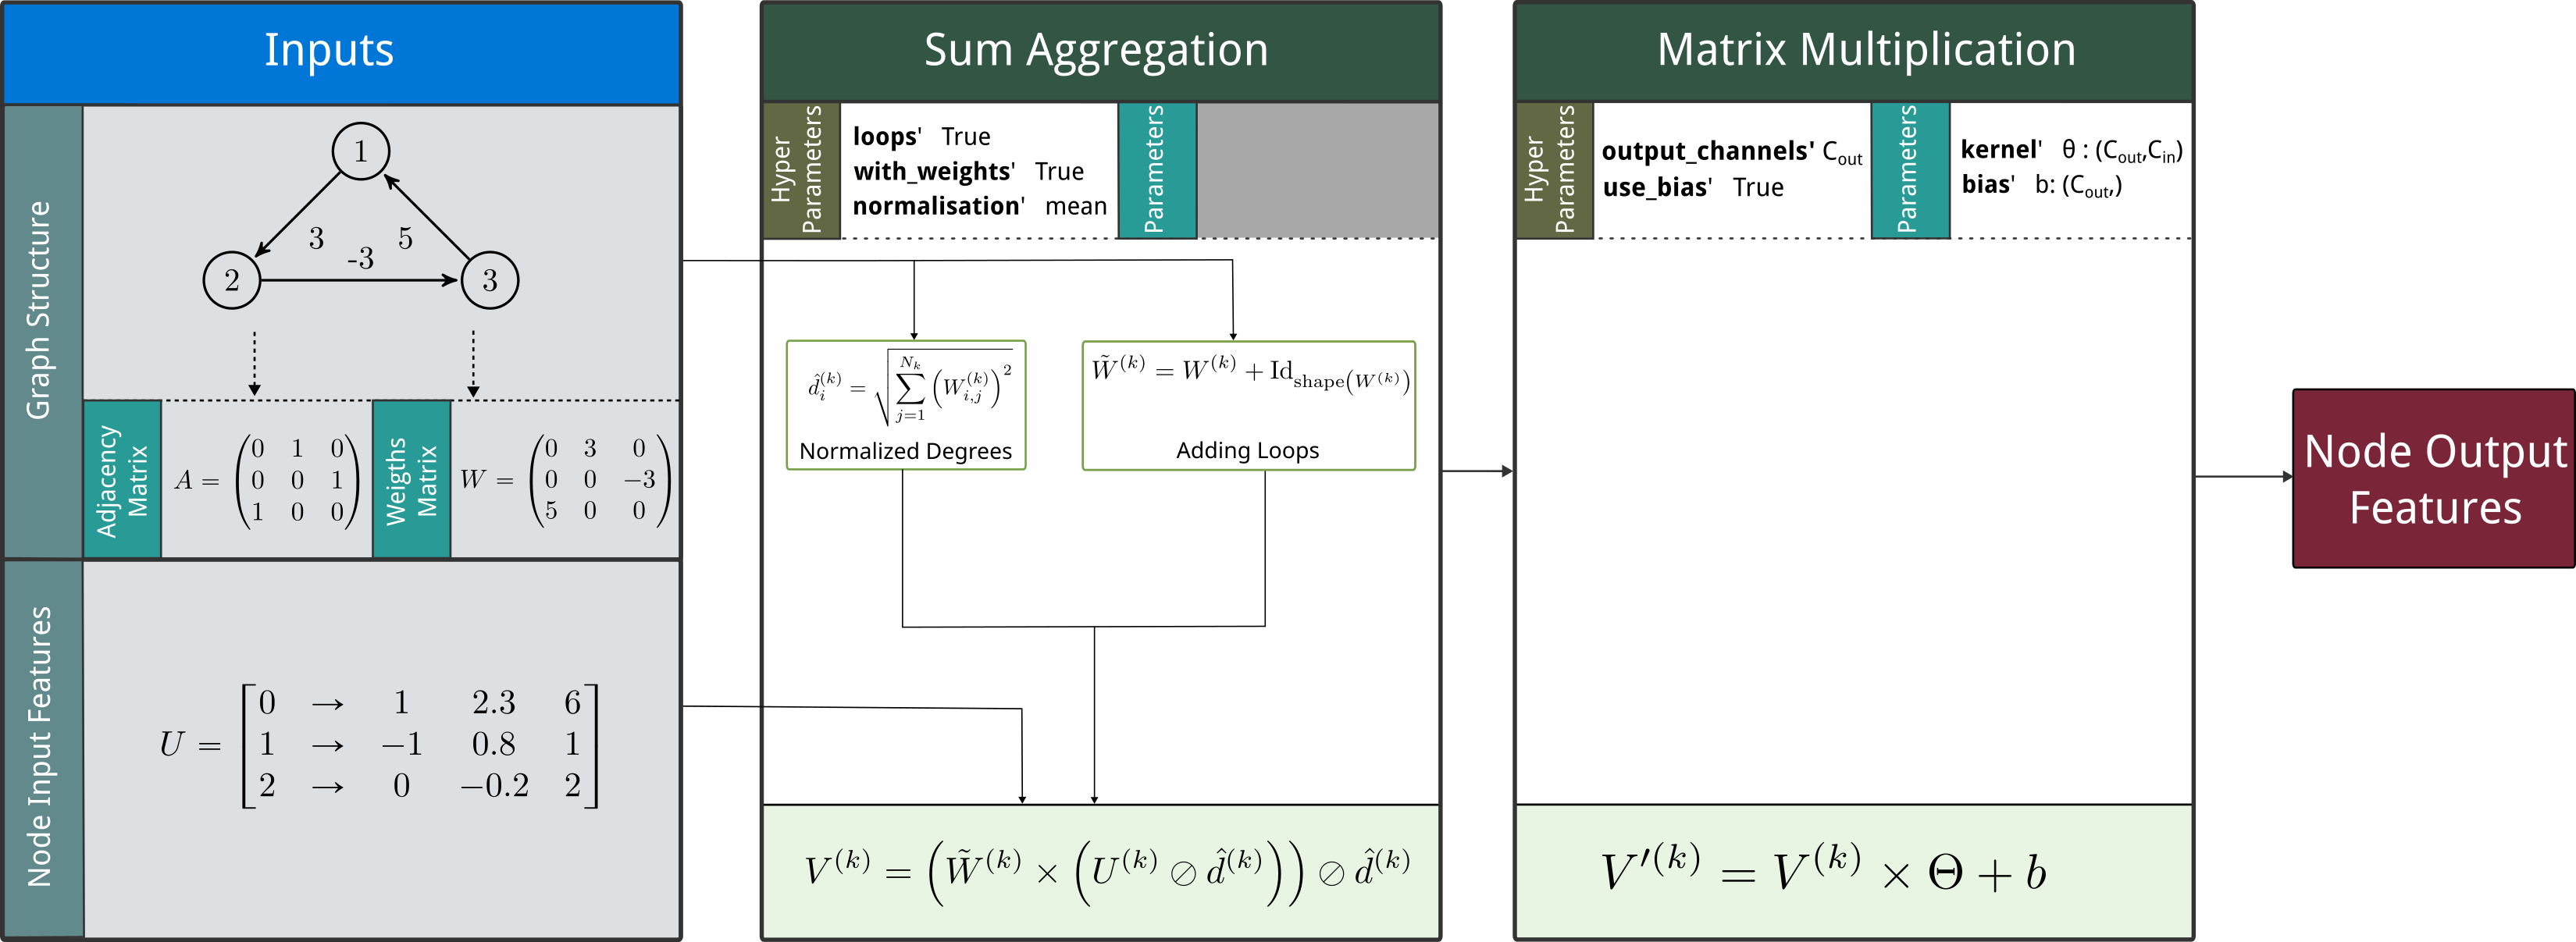
\includegraphics[width=1.2\textwidth]{Figures/WGCN.png}}
	\caption{Weighted Graph Convolutional Network}
	\label{fig:WGCN}
\end{figure}
\FloatBarrier
The \textbf{WGCN} operator exhibits the desired properties described on \ref{section:ModelDesign:Properties}, except property  \ref{section:ModelDesign:Properties:Invariance}.
\subsection{Preprocessing Block}
\begin{figure}[H]
	\noindent
	
	\makebox[\textwidth]{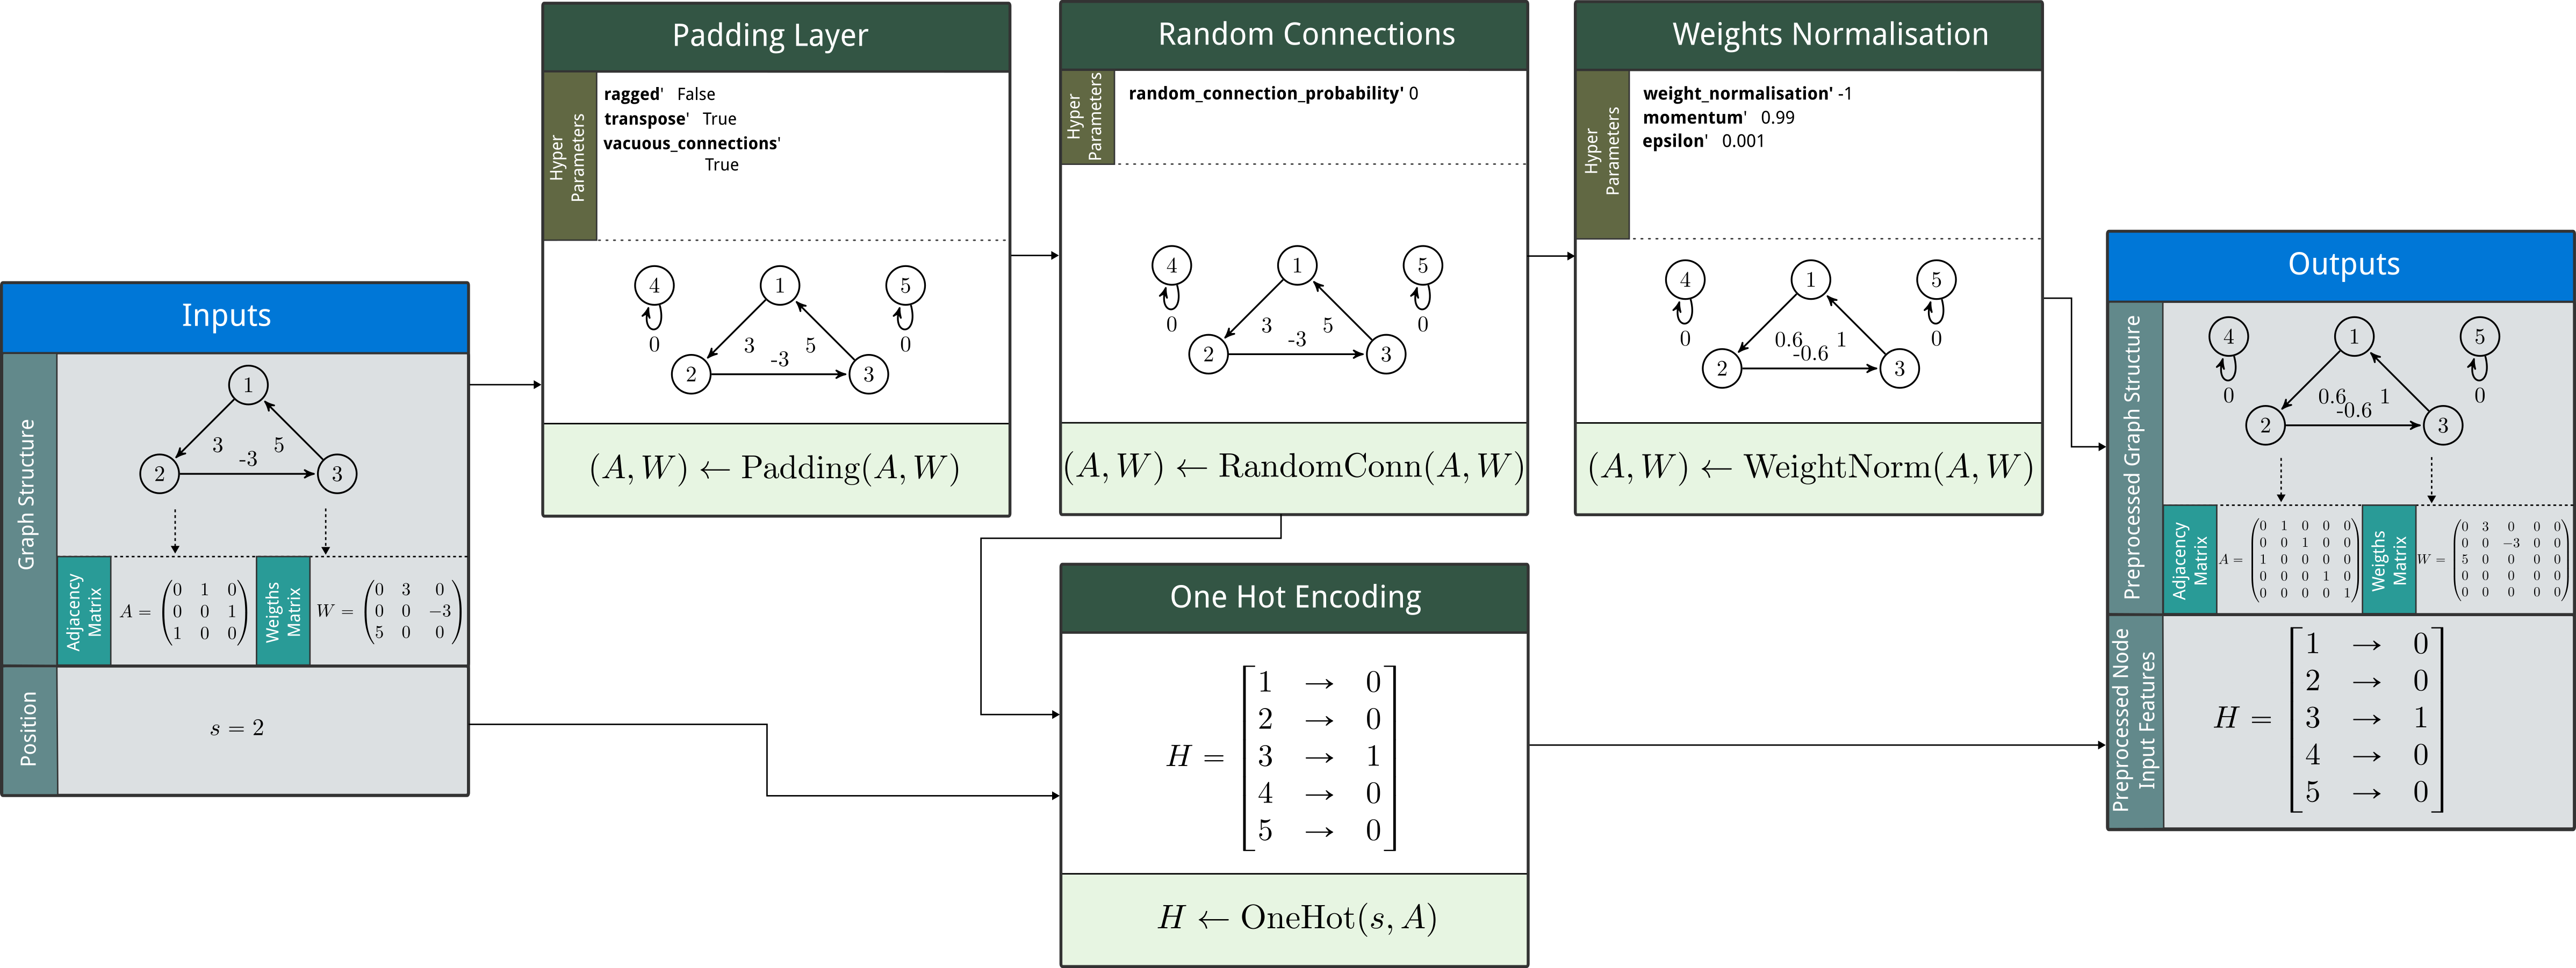
\includegraphics[width=1.2\textwidth]{Figures/PreprocessingBlock.png}}
	\caption{Preprocessing Block}
	\label{fig:PreprocessingBlock}
\end{figure}
\subsection{Convolutional Block}
Each intermediate block is composed of a graph convolution, and then a batch normalisation operator, as described by the figure below:
\begin{figure}[H]
	\noindent
	
	\makebox[\textwidth]{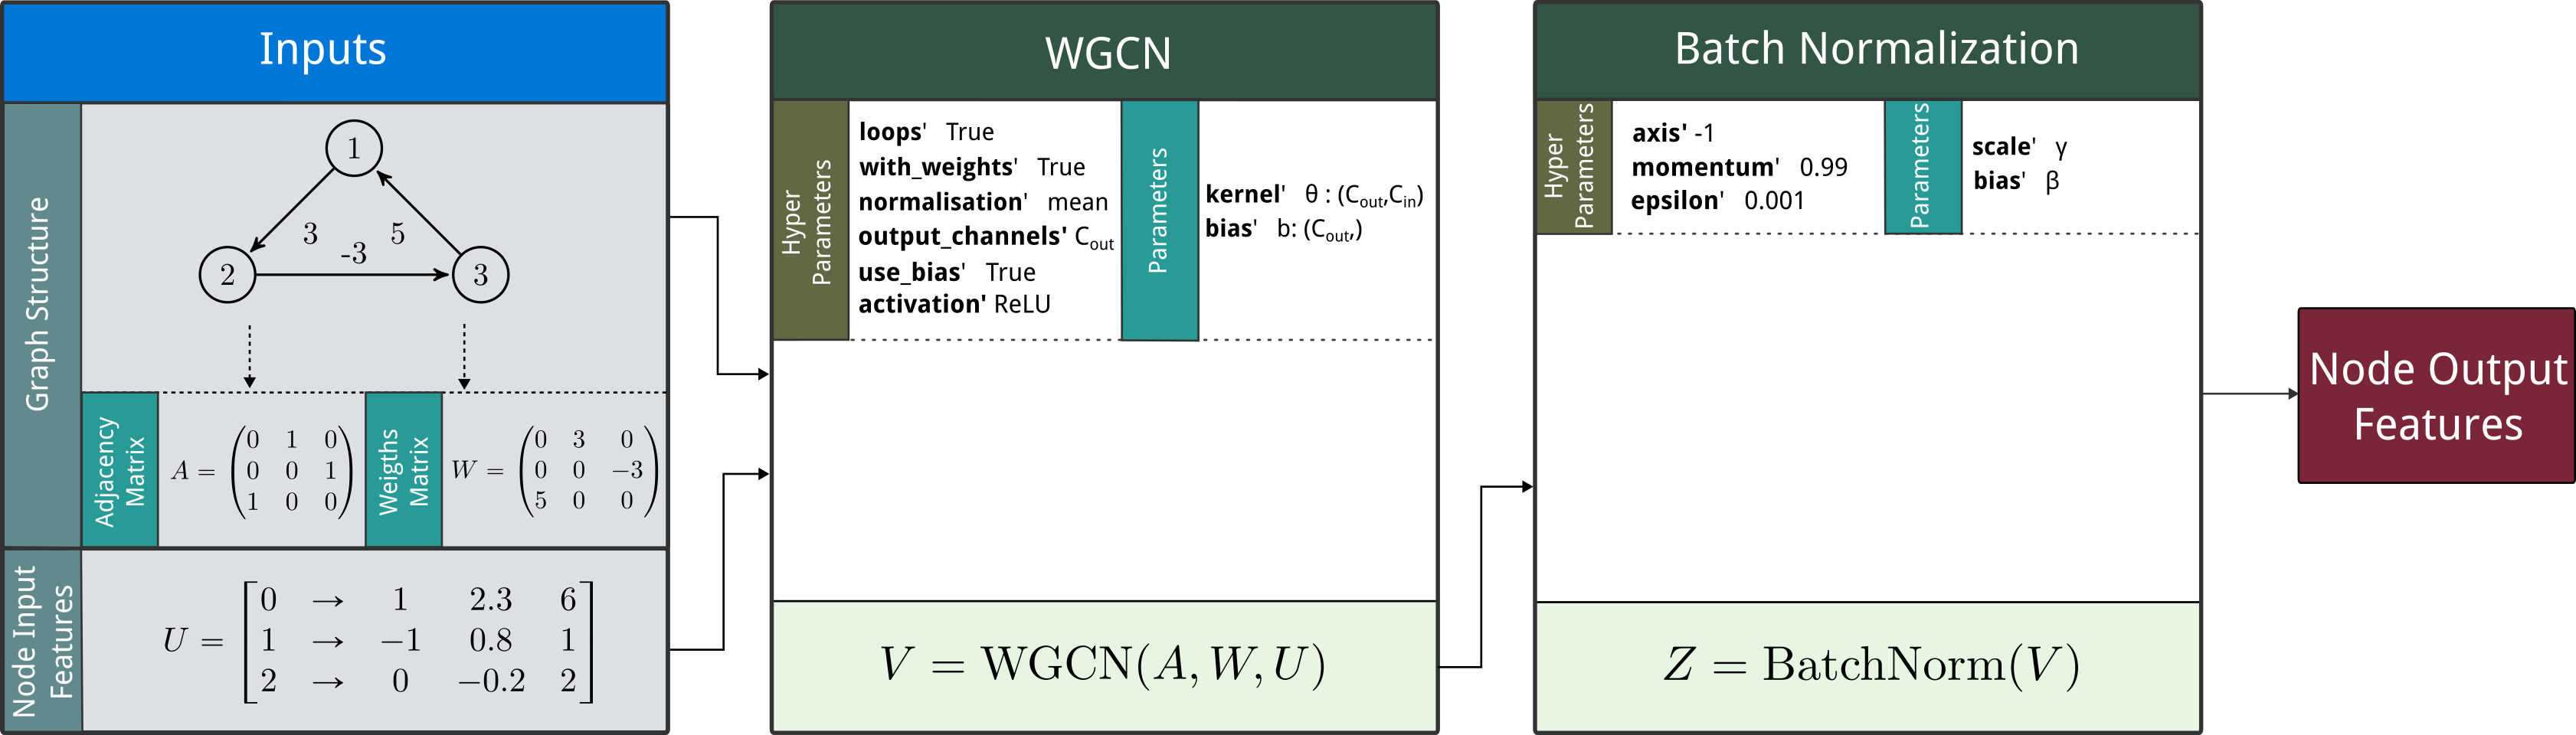
\includegraphics[width=1.2\textwidth]{Figures/ConvolutionalBlock.png}}
	\caption{Graph Convolutional Block}
	\label{fig:ConvolutionalBlock}
\end{figure}
\subsection{Prediction Block}
\begin{figure}[H]
	\noindent
	
	\makebox[\textwidth]{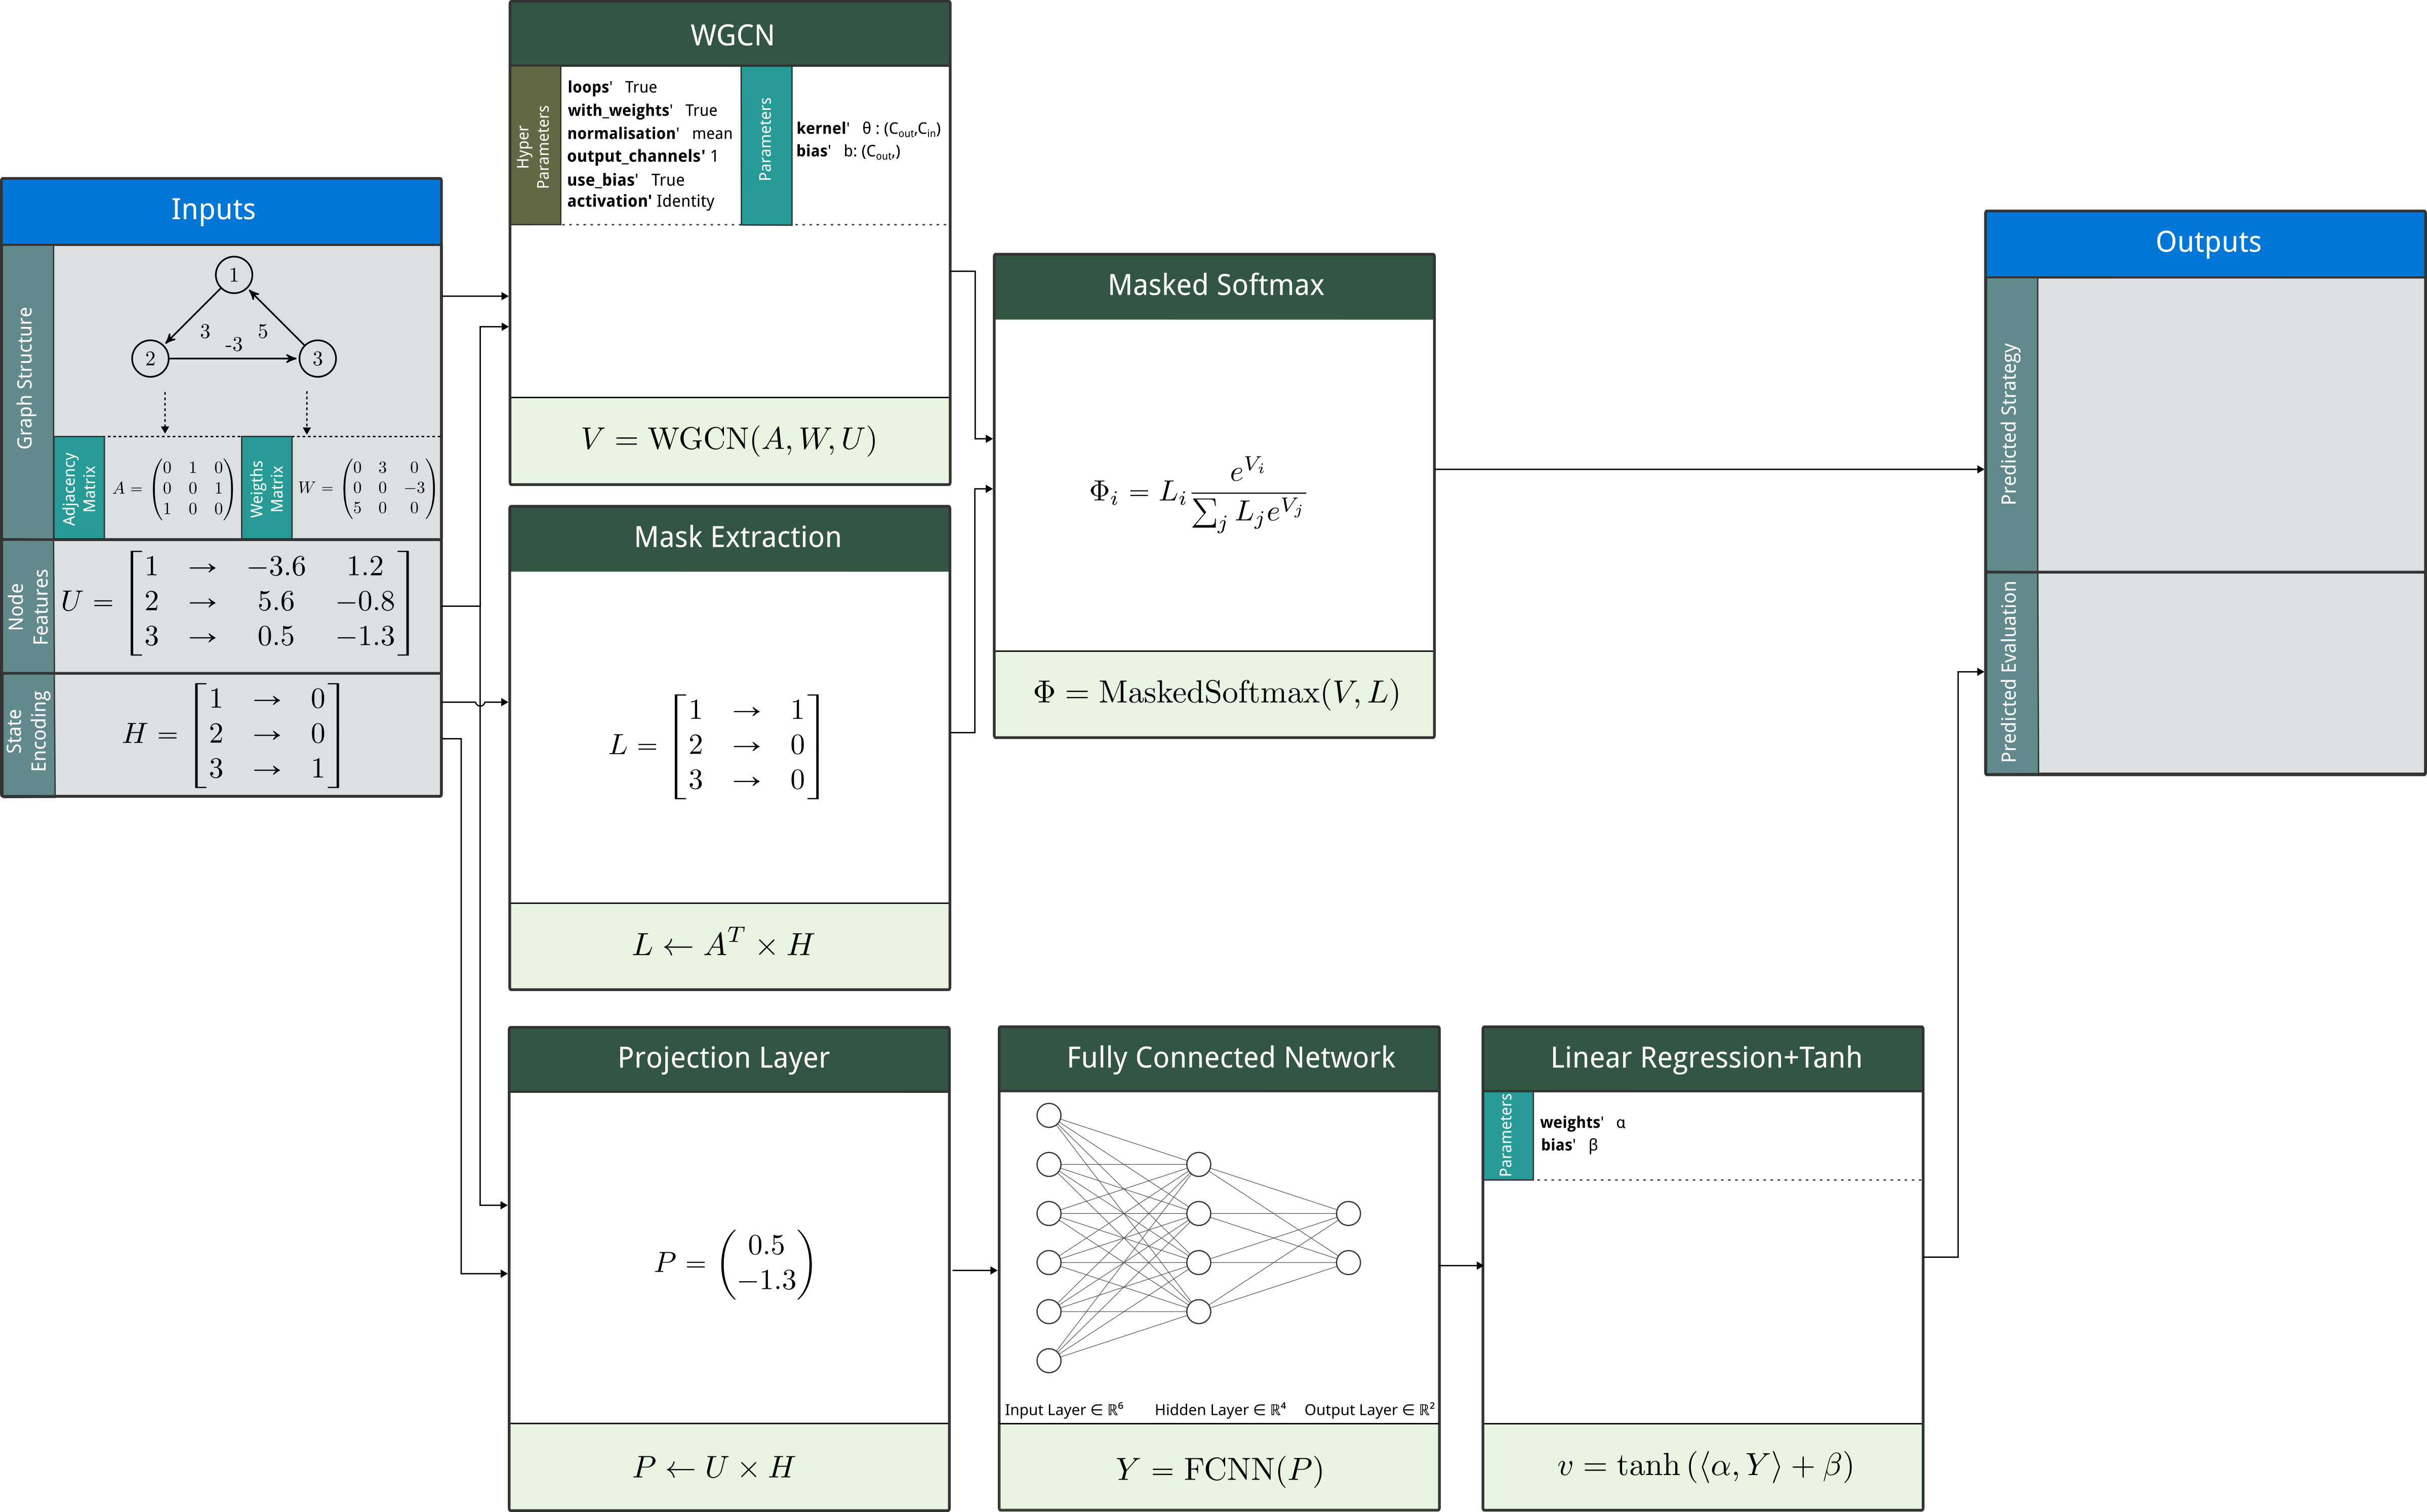
\includegraphics[width=1.2\textwidth]{Figures/PredictionBlock.png}}
	\caption{Graph Convolutional Block}
	\label{fig:PredictionBlock}
\end{figure}
\subsection{Model Architecture}
Putting all building block together, we designed a model that takes arbitrary graphs, encode them, predicts the strategy and the evaluation of the position.
\newline This is detailed by the figure below:
\newpage
\begin{landscape}

	\begin{figure}[H]
	\centering
		
		{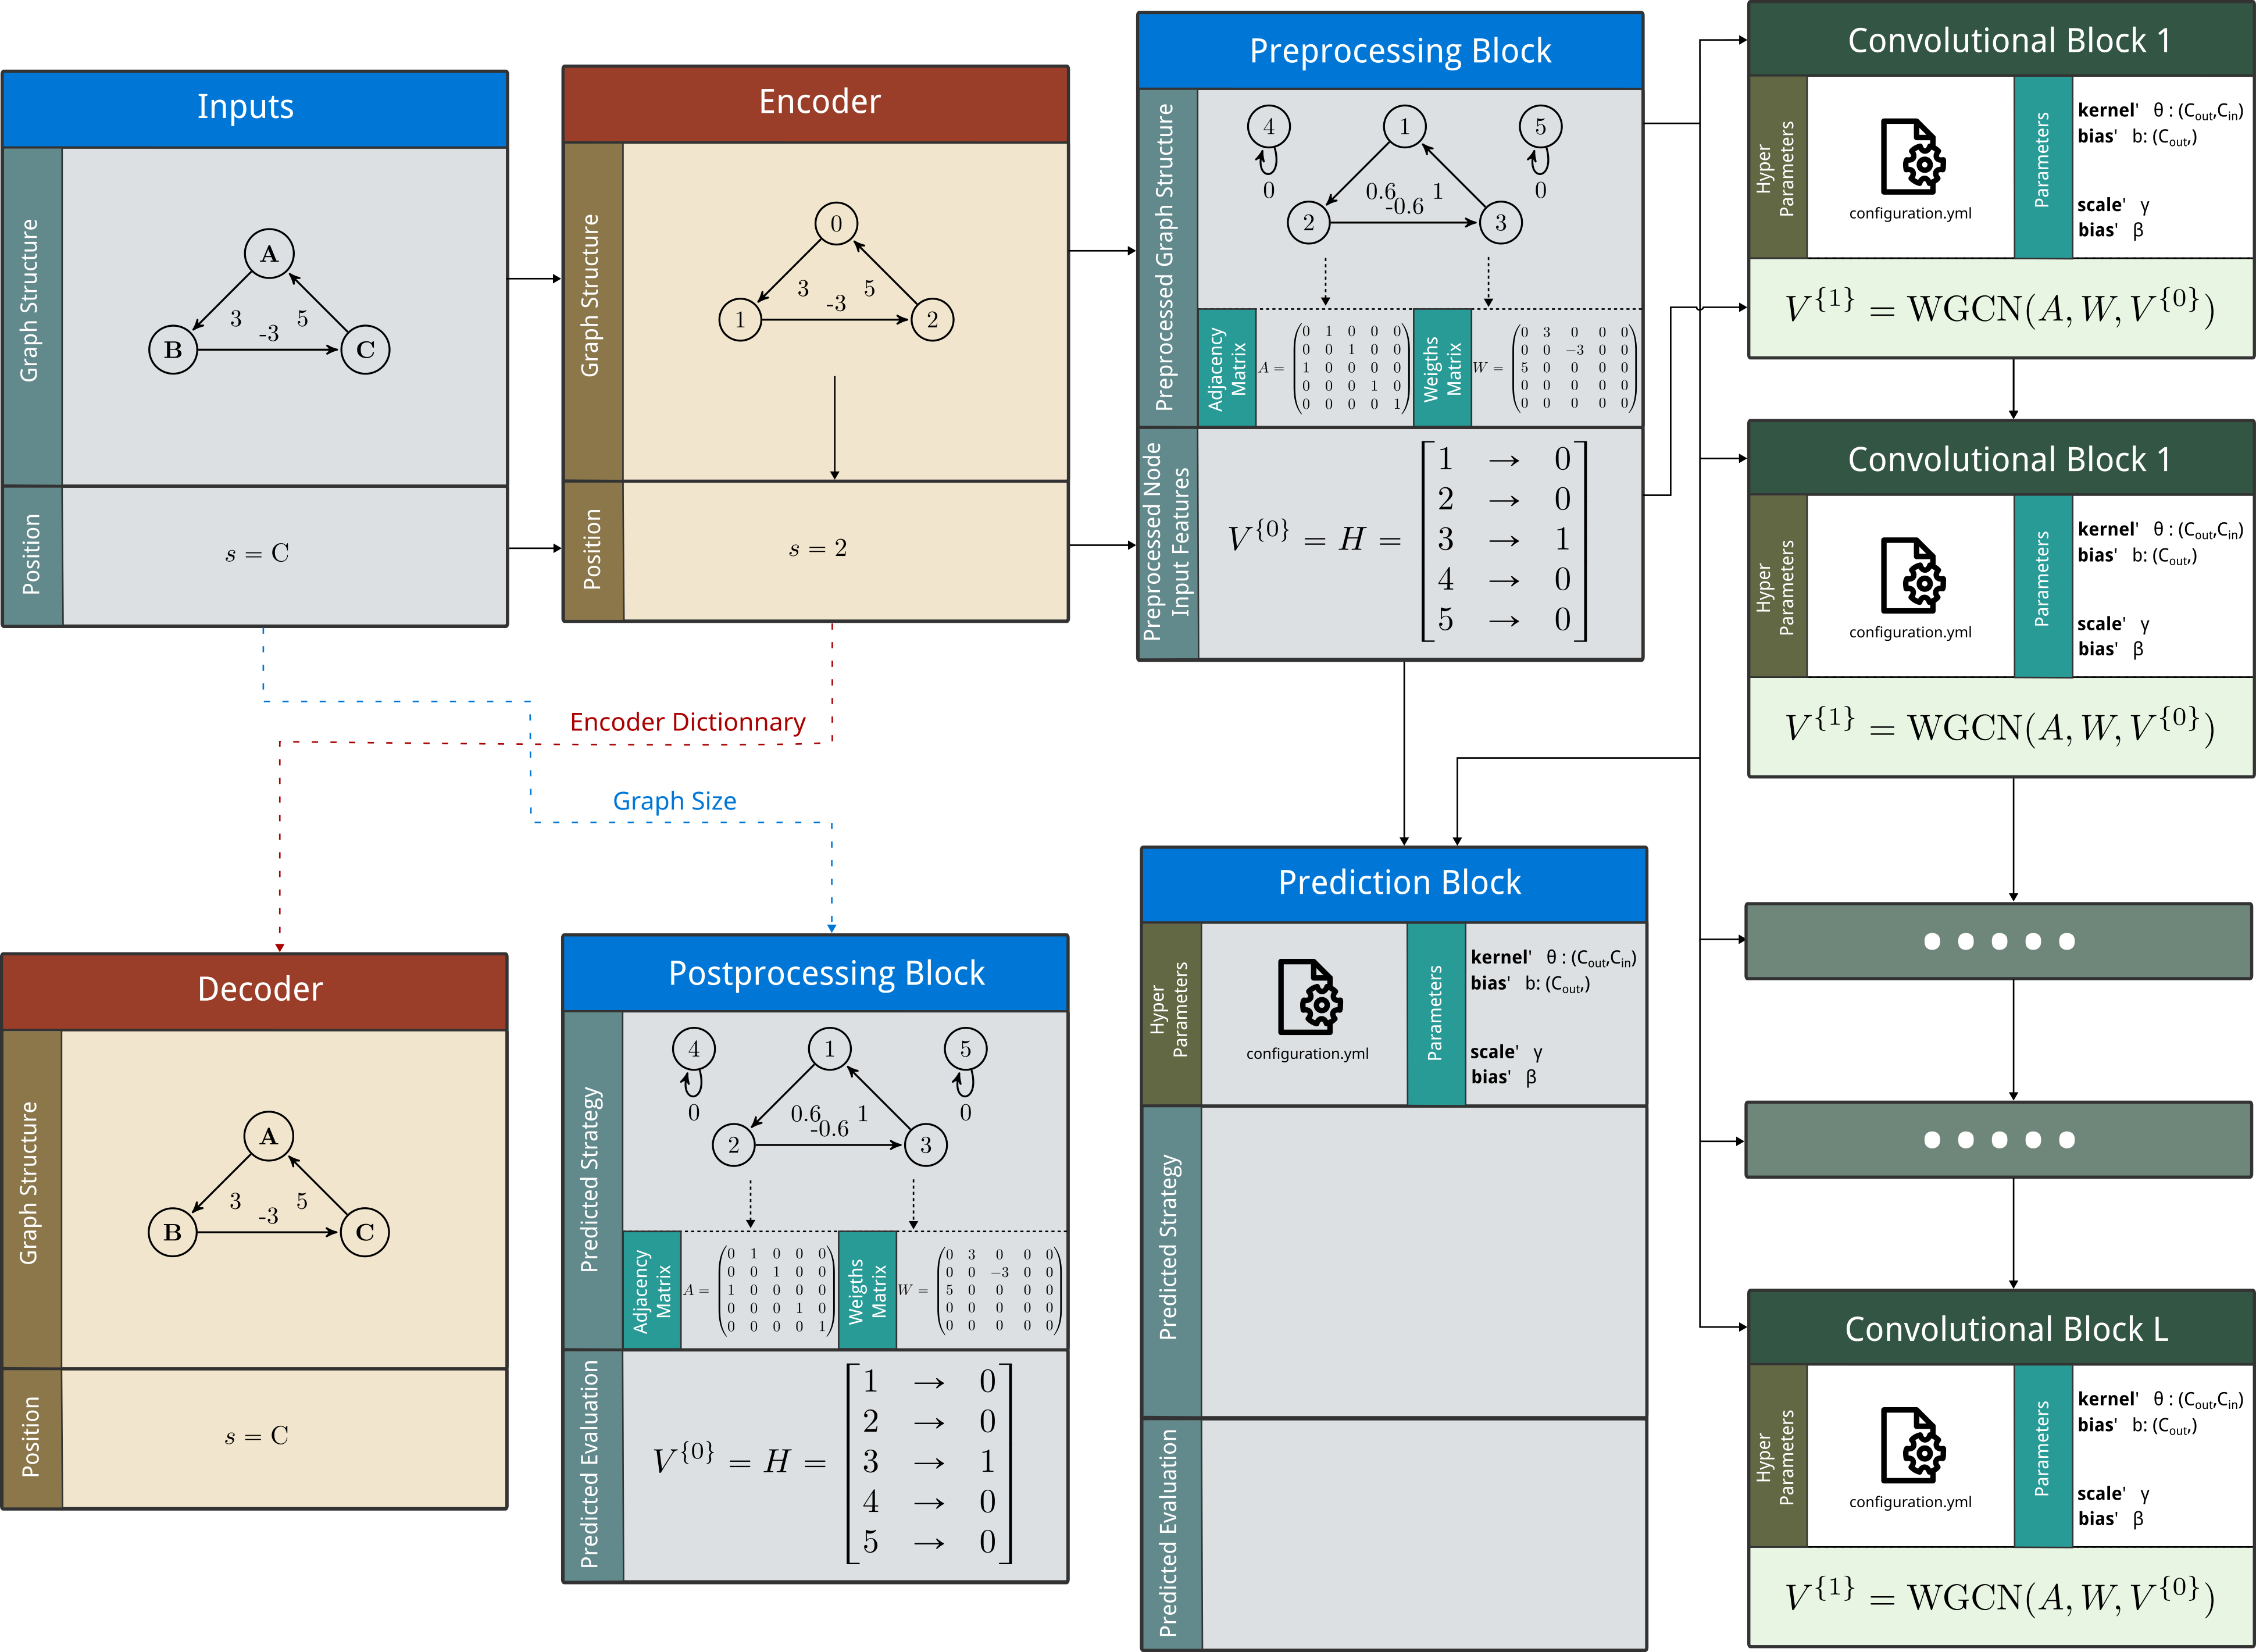
\includegraphics[height=0.95\textheight]{Figures/Architecture.png}}
		\caption{Model Architecture}
		\label{fig:ModelArchitecture}
	\end{figure}
	
\end{landscape}
